\documentclass{article} % For LaTeX2e
\usepackage{nips12submit_e,times}
%\documentstyle[nips12submit_09,times,art10]{article} % For LaTeX 2.09

\def\argmax{\operatornamewithlimits{arg\max}}

\title{Exact Symbolic Dynamic Programming for Continuous POMDPs}


\author{
%Zahra Zamani \\
%ANU & NICTA\\
%Canberra, Australia \\
%\texttt{zahra.zamani@anu.edu.au} \\
%\And
%Coauthor \\
%Affiliation \\
%Address \\
%\texttt{email} \\
%\AND
%Coauthor \\
%Affiliation \\
%Address \\
%\texttt{email} \\
%\And
%Coauthor \\
%Affiliation \\
%Address \\
%\texttt{email} \\
%\And
%Coauthor \\
%Affiliation \\
%Address \\
%\texttt{email} \\
%(if needed)\\
}

% The \author macro works with any number of authors. There are two commands
% used to separate the names and addresses of multiple authors: \And and \AND.
%
% Using \And between authors leaves it to \LaTeX{} to determine where to break
% the lines. Using \AND forces a linebreak at that point. So, if \LaTeX{}
% puts 3 of 4 authors names on the first line, and the last on the second
% line, try using \AND instead of \And before the third author name.

\newcommand{\fix}{\marginpar{FIX}}
\newcommand{\new}{\marginpar{NEW}}

%\nipsfinalcopy % Uncomment for camera-ready version

\begin{document}

\maketitle

\begin{abstract}
Decision-theoretic planning problems try to find the optimal sequence of actions for a given environment. Using continuous models in such problems is naturally closer to the real-world. Partially Observable MDPs model uncertain environments where the underlying state is not be fully observable. 

While previous work have provided solutions for discrete states and/or observations, here we define the first exact solution to both continuous state and observations. This symbolic dynamic programming approach avoids enumerating the state and observation space providing solutions for our general discrete and continuous partially observable MDP. The main contribution of this paper is to use continuous states with discrete observations and extending it to continuous observations by defining relevant observation partitions associated with each state partition. This allows us to perform the Bellman backup operation efficiently. We address the problems in POMDP continuous planning and solutions to solve them symbolically. %To compactly represent the exact value functions Affine algebraic decision diagrams are used. 
\end{abstract}

\section{Introduction}
% Write intro here

The following example is used throughout the paper to help better understand the definitions. 

\textbf{Example} \textsc{(Power Plant)}
\emph{The steam generation system of a power plant aims to provide hot steam to the steam turbine which in turn produces electricity. Feed-water is exposed to heat in the tubes leading to the water tank . Evaporating the water is performed under specific pressure and temperature inside the attached water tubes. 
Mixing water and steam pressures makes reading tank levels and temperatures very hard and uncertain. For this reason, the process is modeled using POMDP in the literature. The temperature is assumed to be a continuous variable that is not observed. Noisy observations of the temperature are used to decide on the action of closing or opening the valve.}

Most work in the literature have assumed discretization of the state and observation space ~\cite{steam2}. Here we take a continuous approach using the DC-POMDP framework.

\section{DC-POMDP Model} 
%%%% no need to define DC-MDP
We assume familiarity with MDPs and introduce Discrete and Continuous Partially Observable MDPs as an extension to Discrete and Continuous State MDPs ~\cite{sanner_uai11}. A Discrete and Continuous partially observable MDP (DC-POMDP) is a tuple $\langle
\mathcal{S},\mathcal{A},\mathcal{O},\mathcal{T},\mathcal{R},\mathcal{Z},\gamma,h \rangle$. 
States are represented by vectors of $(\vec{d_s},\vec{x_s}) = ( d_{s_1},\ldots,d_{s_n},x_{s_1},\ldots,x_{s_m} )$ where each $d_{s_i} \in \{ 0,1 \}$ ($1 \leq i \leq n$) is a discrete boolean and each $x_{s_j} \in  \mathbb{R}$ ($1 \leq j \leq m$) is a continuous variable. Actions are presented by a finite set of actions $\{ a_1, \ldots, a_p \}$. We define discrete and continuous observations by the vector $(\vec{d_o},\vec{x_o}) = ( d_{o_1},\ldots,d_{o_n},x_{o_1},\ldots,x_{o_m} )$ where each $d_{o_i} \in \{ 0,1 \}$ ($1 \leq i \leq n$) is boolean and each $x_{o_j} \in \mathcal{R}$ ($1 \leq j \leq m$) is a continuous variable. 

Three functions are required for modeling DC-POMDPs: (1) $\mathcal{T}: \mathcal{S} \times \mathcal{A} \times \mathcal{S} \rightarrow  [ 0, 1 ]$ a Markovian transition model defined as the probability of the next state given the action and previous state%$P(\vec{d}',\vec{x}'|\cdots,a)$
; (2)  $\mathcal{R}:\mathcal{S}\times\mathcal{A} \rightarrow \mathbb{R}$ a reward function which returns the immediate reward of taking an action in some state and (3) an observation function defined as $\mathcal{Z} : \mathcal{S} \times \mathcal{A} \times \mathcal{O} \rightarrow [ 0, 1 ]$  which gives the probability of an observation given the outcome of a state after executing an action.  A discount factor $\gamma, \; 0 \leq \gamma \leq 1$ is included in the model to account for future rewards in higher horizons.

%%%% forms of transition, observation and reward function
To define the transition function, we use the fact that the state variables of this POMDP can be factored into a Dynamic Bayesian Network (DBN). Not allowing synchronic arcs between the discrete and continuous variables defines their joint transition to be independent: 

{\footnotesize
\begin{equation}
P(\vec{d_s}',\vec{x_s}'|\vec{d_s},\vec{x_s},a) = 
\prod_{i=1}^n P(d_{s_i}'|\vec{d_s},\vec{x_s},a) \prod_{j=1}^m P(x_{s_j}'|\vec{d_s},\vec{d_s}',\vec{x_s},a). \nonumber 
\end{equation}}
The joint observation function can also be defined considering the direct correspondence between the state and observation variables:
{\footnotesize
\begin{equation}
P(\vec{d_o},\vec{x_o}|\vec{d_s},\vec{x_s},a) = 
\prod_{i=1}^n P(d_{o_i}|d_{s_i},a) \prod_{j=1}^m P(x_{o_j}|x_{s_j},a). \nonumber 
\end{equation}}

The \emph{binary} variables are represented using conditional probability functions (CPF) in the form of $P(d_i'|\vec{d},\vec{x},a)$. For \emph{continuous} variables
the CPF $P(x_j'|\vec{d},\vec{d'},\vec{x},a)$ is represented by \emph{piecewise
linear equations} (PLEs) that are first-order Markov and deterministic, i.e. the probabilities are encoded using the Dirac $\delta[\cdot]$ function.  The reward function $R(\vec{d},\vec{x},a)$ is set to be any general piecewise linear  function that could facilitate pruning for space efficiency via bilinear solvers. 

For the \textsc{Power Plant} example, the temperature $t_s \in \mathbb{R}$ is modelled as the continuous state variable. Noisy observation of the temperature $t_o \in \mathbb{R}$ is used to help decide the optimal action to either open or close the pressure valve $a \in \{open,close\}$. 
For the transition probability, we use the Dirac function to model the deterministic equations. We can also define stochasticity in the transition model using boolean random variables that are sampled stochastically.  The reward function can be any linear function of the state or action. Going above a threshold temperature (e.g. $T=10$) will cause an explosion in the plant when trying to close the valve which results in the negative reward of $-1000$. Staying below this temperature is safe and will produce electricity an gain the reward of $100$. The reward of an open valve is $-1$.
\begin{align}
P(t_s'|\vec{t_s},a)= \delta\left[ t_s' - 
\begin{cases}
 (a=open) &: t_s - 5 \\ 
(a \neq open) &: t_s + 7 \\
\end{cases}
\right]\nonumber
, 
R(t_s,a) = 
\begin{cases}
 (a=open) &: -1 \\
(a \neq open)\wedge (t_s>T) &: -1000 \\
(a \neq open)\wedge \neg(t_s>T) &: 100 \\
\end{cases}\nonumber
\end{align}
%contribution? 
This example will try to maximize its reward using observations on the temperature. The observations recieved before closing the plant to a safe temperature are therefore critical.  For the observation model we begin with a discrete model for two observations $t_{o_1},t_{o_2}$ such as the following:  
\begin{align}
P(t_{o_1}|t_s',open) = 
\begin{cases}
 \delta\left[ t_s <= 15 \right] &: 0.9 \\
 \delta\left[ \neg (t_s <= 15)\right] &: 0.1 \\
\end{cases}\nonumber
, 
P(t_{o_2}|t_s',open) = 
\begin{cases}
 \delta\left[ t_s <= 15 \right] &: 0.1 \\
 \delta\left[ \neg (t_s <= 15)\right] &: 0.9 \\
\end{cases}\nonumber
\\
P(t_{o_1}|t_s',close) = 
\begin{cases}
 \delta\left[ t_s <= 15 \right] &: 0.1 \\
 \delta\left[ \neg (t_s <= 15)\right] &: 0.8 \\
\end{cases}\nonumber
,
P(t_{o_2}|t_s',close) = 
\begin{cases}
 \delta\left[ t_s <= 15 \right] &: 0.9 \\
 \delta\left[ \neg (t_s <= 15)\right] &: 0.2 \\
\end{cases} \nonumber
\end{align}

After defining the solution to the discrete observation with a continuous state DC-POMDP, we can extend this to consider continuous observations using a continuous uniform noise distribution which is more realistic in many domains. For a certain interval, the probability is a fixed number, while it is zero elsewhere. The integral of the uniform distribution should sum to one. 
\begin{align}
P(t_o|t_s',open) = 
\begin{cases}
 (t_o>t_s-5) \wedge (t_o<t_s+5) &: 0.1 \\
 \neg((t_o>t_s-5) \wedge (t_o<t_s+5)) &: 0 \\
\end{cases}\nonumber
\end{align}

Next we define the general solution to solving DC-POMDPs. 

\section{DC-POMDP solution}
The DC-POMDP will choose actions in order to compute an optimal plan over time. This plan is the policy $\pi$ of the agent  depending on the history of actions and observations over a Markovian state. In the partially observable case where there is uncertainty on the states, the policy is a function over a continuous set of probability distributions over $|\mathcal{S}|$. Observations don't provide a unique state therefore the probability of the state is stored as the belief state $b$.

 At any of the horizon steps, a DC-POMDP policy $\pi(b)$ is defined as the iterative plan on executing an action and observing all probable outcomes of the set of observations from the $(h-1)$-step. The belief state is updated after this according to the Bayes rule: $\sum_{d_s}\int_{x_s} b(xd_s)T(xd'_s,xd_s,a)Z(xd'_s,xd_o,a)$  where for simiplicity we use ($xd_s = x_s,d_s$) and ($xd_o=x_o,d_o$).
The optimal policy is defined over the belief state as the sum of the expected discounted rewards over horizon $h$ starting with belief $b_0$.
\begin{equation}
V^h_{\Pi^*}(\vec{b}) = E_{\pi^*} \left[ \sum_{h=0}^{H} \gamma^t \cdot r_h \Big| \vec{b}_0 = \vec{b} \right]\nonumber
\end{equation}
%The next section provides the mathematics required to solve this equation in DC-POMDPs.
%%%%%%%%%%%%%%%%%%%%%%%%%%%%%%%%%%%%%%%%%%%%%%%%%%%%%%%%%%%%%%%%%%%%%%%%
% Figure 1 - policy tree
\begin{figure}[t!]
%\vspace{-1mm}
\begin{center}
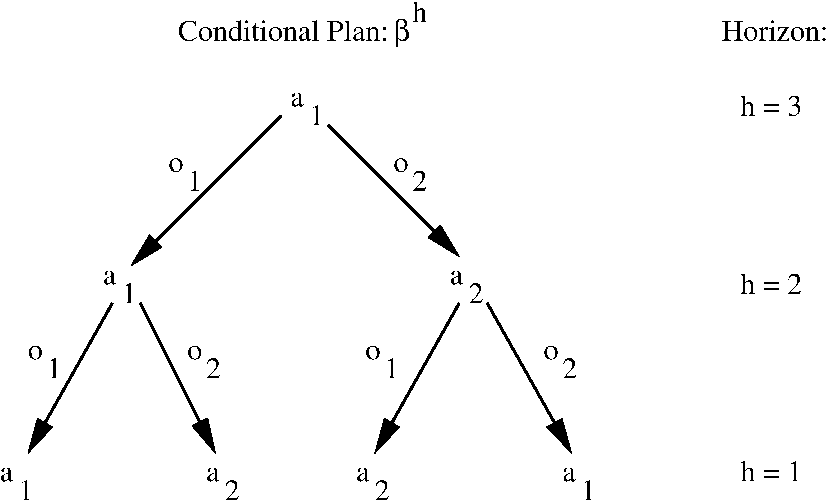
\includegraphics[width=0.4\textwidth]{pics/cond_plan2.pdf}
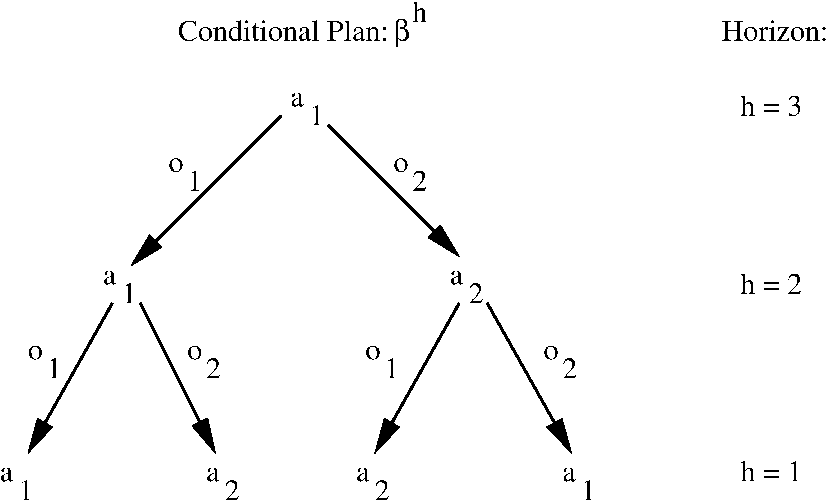
\includegraphics[width=0.4\textwidth]{pics/cond_plan2.pdf}
\end{center}
\vspace{-2mm}
\caption{\footnotesize Left: Example conditional plan $\beta^h$ for discrete observations. Right: The optimal value function for \textsc{Power Plant}
as a decision diagram: 
the \emph{true} branch is solid, the \emph{false}
branch is dashed.}
\label{fig:cond_plan}
\vspace{-1mm}
\end{figure}
%%%%%%%%%%%%%%%%%%%%%%%%%%%%%%%%%%%%%%%%%%%%%%%%%%%%%%%%%%%%%%%%%%%%%%%%
%%%%%%%%%%%%%%%%%%%%%%%%%%%%%%%%%%%%%%%%%%%%%%%%%%%%%%%%%%%%%%%%%%%%%%%%%%%
%\begin{figure}[t]
%\begin{center}
%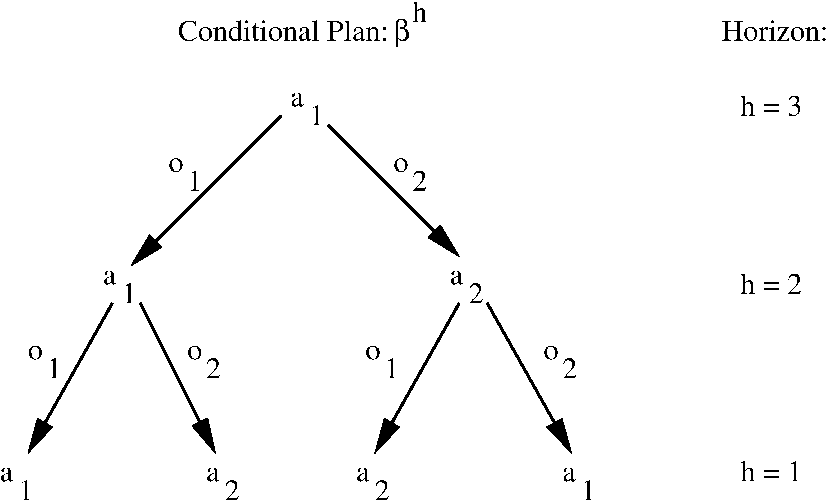
\includegraphics[width=0.4\textwidth]{pics/cond_plan2.pdf}
%\end{center}
%\vspace{-3mm}
%\caption{%\footnotesize 
%The optimal value function for \textsc{Power Plant}
%as a decision diagram: 
%the \emph{true} branch is solid, the \emph{false}
%branch is dashed.} 
%\end{figure}
%%%%%%%%%%%%%%%%%%%%%%%%%%%%%%%%%%%%%%%%%%%%%%%%%%%%%%%%%%%%%%%%%%%%%%%%%%%
%\subsection{Dynamic Programming solution} 
Solving the value function for the optimal policy is performed using Dynamic programming algorithms such as value iteration. 
The decision at each time step is to pick an action based on past actions and observations. The possible set of conditional plans $\beta^h$ correspond to a decision tree. Figure 1 left, shows the decision tree for the simple case of three horizons with discrete observations. It represents a conditional plan consisting of an action and two possible observation strategies. For continuous observations, conditional plans are decision trees with infinitely many branches. In our solution we show that instead of a policy tree with infinite branches, we can create partitions based on relevant observation values, resulting in a policy tree similar to that of figure 1. %From here on we assume this finite set of observation partitioning as $\mathcal{O}$.

We define the value iteration algorithm for discrete observations and discrete states that finds the optimal value for each horizon starting with an initial belief. Although the number of belief states is infinite, the optimal value function for $h$ is proven to be a piecewise linear and convex function of the belief state \cite{smallwoodSondik}. The optimal value function is the maximum value over a finite set of alpha vectors  $\alpha^h_i$:%that define the hyperplanes:
\begin{equation}
V^h_{\Pi^*}(\vec{b}) = \max_{\alpha^h_i \in \Gamma^h} \alpha^h_i \cdot \vec{b}
\end{equation}
where the belief states $\vec{b}$ and each $\alpha^h_i \in \Gamma^h$ are of dimension $|\mathcal{S}|$. At each of the $h$-steps the value function is parameterized by the set of  $\alpha$-vectors that partition the belief state. 
At a particular belief point, we can compute the next value function: 
\begin{align*}
V^{h+1}(b) = \max_a \left( b \cdot r_a + \gamma \sum_o p(xd_o|a,b)V^h(b|xd_o,a)\right)\nonumber
\end{align*}
Replacing the previous iteration value with (3) and also updating the belief after executing action $a$ and observing $xd_o$ results in the following equation: 
\begin{align*}
V^{h+1}(b) = \max_a \left( b \cdot r_a + 
\gamma \sum_o \max_{\langle g^h_{a,o,j} \rangle_j}  b \cdot g^h_{a,o,j} \right)\nonumber
\end{align*}
where $r_a = r(x_s,d_s,a)$ and  
$g^h_{a,o,j} =  \int_{x_{s'}} \sum_{d_{s'}} p(xd_o|xd'_s,a)p(xd'_s|xd_s,a) \alpha^h_j(xd'_s)$

Calculating all possible ways of building the value function independent of a certain belief state can define the optimal value function. To derive the $\Gamma$-set of all possible $\alpha$-vectors for each horizon, we use the value iteration algorithm from (Monahan)~\cite{monahan82}. 
Initializing  $\alpha^0_1 = \vec{0}$ and $\Gamma^0 = \{ \alpha^0_1 \}$, $\Gamma^h$ is obtained from $\Gamma^{h-1}$ using the backup operation defined in (4):\footnote{The $\textrm{\large $\boxplus$}$ of sets is defined as 
$\textrm{\large $\boxplus$}_{j \in \{ 1,\ldots, n \} } S_j = S_1 \textrm{\large $\boxplus$} \cdots \textrm{\large $\boxplus$} S_n$ where the pairwise cross-sum $P 
\textrm{\large $\boxplus$} Q = \{ \vec{p} + \vec{q} | \vec{p} \in P, \vec{q} \in Q \}$.}
\begin{align}
\Gamma^{h}_a   &= r_a + \gamma \textrm{\large $\boxplus$}_{o \in \mathcal{O}} \left\{ g^h_{a,o,j}(\cdot) \right\}_j ;  \forall \alpha^{h-1}_{j} \in \Gamma^{h-1}  \\
\Gamma^h  &= \bigcup_a \Gamma^h_a 
\end{align}
Each action-dependent $\Gamma$ sums over the possible set of $g^h_{a,o,j}(\cdot)$ given an observation model to derive discrete observations $xd_o$ and for all $\alpha^{h-1}_{j} \in \Gamma^{h-1} $. The value $g^h_{a,o,j}(\cdot)$ is computed by summing over all states given the probability functions and previous $\alpha$-vectors.  
For each horizon, the optimal $\alpha$-vector is obtained from the maximum over all $\alpha$-vectors: 
$\alpha^* = \argmax_{\alpha^h_i \in \Gamma^h} \alpha^h_i \cdot b $

Here the cross-sum operation takes the set of $\alpha$ -vectors for each observation and produces a sum over vectors that depends on the number of previous iteration vectors. Thus the $\alpha$-vector set grows exponentially in the number of observations, i.e., $|\Gamma^{h}| = |\mathcal{A}||\Gamma^{h-1}|^{|\mathcal{O}|}$ during the cross-sum operation. For this reason even for a small number of discrete observations, tractable solutions may be hard to define. Here we do not restrict our observations to discrete ones, but extend it to a fully continuous approach where continuous observations and states are allowed in the DC-POMDP. We use the number of  observation partitions $|\mathcal{O}|$ as the branching factor in the policy tree. We present the symbolic value iteration algorithm in the case of continuous observations using relevant observation partitioning of this continuous space. 

\section{Symbolic Dynamic Programming} 
Dynamic programming provides exact solutions to POMDP problems for small domains. As the domain grows, fully enumerating the state, action and observation space leads to intractable solutions even for low horizons. Avoiding this enumeration often requires approximating the solutions. We claim an exact solution using symbolic dynamic programming. The SDP solution for fully observable domains has been presented in \cite{sanner_uai11} %using piecewise constant functions
Our symbolic algorithm deals with continuous observations and states by generating the relevant observation partition at every time step and performing the backup operation using $\alpha$-vectors. We define the requirements to implement the value iteration algorithm for DC-POMDP. 

\subsection{Case Representation and Extended ADDs}
% operations, max, restrict, substitute
%overview + example plant
The \textsc{Power Plant} example represented all functions using the case structure which can be generally defined as:
{%\footnotesize 
\begin{align}
f = 
\begin{cases}
  \phi_1: & f_1 \\ 
 \vdots&\vdots\\ 
  \phi_k: & f_k \\ 
\end{cases} \nonumber
\end{align}
}
Where $\phi_i$ are disjoint logical formulae defined over the state $(\vec{d},\vec{x})$ with logical ($\land,\lor,\neg$) combinations of boolean variables and inequalities ($\geq,>,\leq,<$) over continuous variables.  
The $f_i$ are function definitions either linear or quadratic in the continuous parameters. 

For \emph{unary operations} such as scalar multiplication $c\cdot f$ (for some constant $c \in \mathbb{R}$) or negation $-f$ on case statements is simply to apply the operation on each case partition $f_i$ ($1 \leq i \leq k$). 

A \emph{binary operation} on two case statements, takes the cross-product of the logical partitions of each case statement and performs the corresponding operation on the resulting paired partitions.  The cross-sum $\oplus$ of two cases is defined as the following:
{\footnotesize 
\begin{center}
\begin{tabular}{r c c c l}
&
\hspace{-6mm} 
  $\begin{cases}
    \phi_1: & f_1 \\ 
    \phi_2: & f_2 \\ 
  \end{cases}$
$\oplus$
&
\hspace{-4mm}
  $\begin{cases}
    \psi_1: & g_1 \\ 
    \psi_2: & g_2 \\ 
  \end{cases}$
&
\hspace{-2mm} 
$ = $
&
\hspace{-2mm}
  $\begin{cases}
  \phi_1 \wedge \psi_1: & f_1 + g_1 \\ 
  \phi_1 \wedge \psi_2: & f_1 + g_2 \\ 
  \phi_2 \wedge \psi_1: & f_2 + g_1 \\ 
  \phi_2 \wedge \psi_2: & f_2 + g_2 \\ 
  \end{cases}$
\end{tabular}
\end{center}
}
\normalsize
Likewise $\ominus$ and $\otimes$ are defined by subtracting or multiplying partition values.  Inconsistent partitions can be discarded when they are irrelevant to the function value.
The next three operations are required in defining the value iteration algorithm. A \emph{symbolic case maximization} is defined as below:
\vspace{-4mm}

{\footnotesize
\begin{center}
\begin{tabular}{r c c c l}
&
\hspace{-7mm} $\mathrm{max} \Bigg(
  \begin{cases}
    \phi_1: \hspace{-2mm} & \hspace{-2mm} f_1 \\ 
    \phi_2: \hspace{-2mm} & \hspace{-2mm} f_2 \\ 
  \end{cases}$
$,$
&
\hspace{-4mm}
  $\begin{cases}
    \psi_1: \hspace{-2mm} & \hspace{-2mm} g_1 \\ 
    \psi_2: \hspace{-2mm} & \hspace{-2mm} g_2 \\ 
  \end{cases} \Bigg)$
&
\hspace{-4mm} 
$ = $
&
\hspace{-4mm}
  $\begin{cases}
  \phi_1 \wedge \psi_1 \wedge f_1 > g_1    : & \hspace{-2mm} f_1 \\ 
  \phi_1 \wedge \psi_1 \wedge f_1 \leq g_1 : & \hspace{-2mm} g_1 \\ 
  \phi_1 \wedge \psi_2 \wedge f_1 > g_2    : & \hspace{-2mm}f_1 \\ 
  \phi_1 \wedge \psi_2 \wedge f_1 \leq g_2 : & \hspace{-2mm} g_2 \\ 
  %\vdots & \vdots
  \phi_2 \wedge \psi_1 \wedge f_2 > g_1    : & \hspace{-2mm} f_2 \\ 
  \phi_2 \wedge \psi_1 \wedge f_2 \leq g_1 : & \hspace{-2mm} g_1 \\ 
  \phi_2 \wedge \psi_2 \wedge f_2 > g_2    : & \hspace{-2mm} f_2 \\ 
  \phi_2 \wedge \psi_2 \wedge f_2 \leq g_2 : & \hspace{-2mm} g_2 \\ 
  \end{cases}$
\end{tabular}
\end{center}
}
\emph{Restriction} takes a function $f$ to restrict only in cases
that satisfy some formula $\phi$, which we write as $f|_{\phi}$.  
This can be done by simply appending $\phi$ to each case partition
as follows:
{\footnotesize
\begin{center}
\begin{tabular}{r c c l}
&
\hspace{-6mm} 
  $f = \begin{cases}
    \phi_1: & f_1 \\ 
   \vdots&\vdots\\ 
    \phi_k: & f_k \\ 
  \end{cases}$
&

&
\hspace{-2mm}
  $f|_{\phi} = \begin{cases}
    \phi_1 \land \phi : & f_1 \\ 
   \vdots&\vdots\\ 
    \phi_k \land \phi : & f_k \\ 
  \end{cases}$
\end{tabular}
\end{center}
}

\emph{Symbolic substitution} simply takes a set $\sigma$ of variables and their substitutions, where
the LHS of the substitution operator $/$ represents the substitution variable and the
RHS of the $/$ represents the expression that should be substituted in its place.
Hence to perform a continuous regression on a more general
representation, we obtain that $\int_{x_j'} P(x_j'|\cdots) V'^{h} dx_j'$
\begin{align*}
    = \begin{cases}
    \phi_1: & V'^{h} \{ x_j' = f_1 \} \\ 
   \vdots&\vdots\\ 
    \phi_k: & V'^{h} \{ x_j' = f_k \}  \\ 
  \end{cases}
\end{align*}


%xadd representation
The data structure of \emph{extended ADD} (XADD)~\cite{sanner_uai11} is used to support
case statements and the required operations.  Here we use continuous SDP for both states and observations in DC-POMDPs. The value functions and $\alpha$-vectors partition into states of equal value, both of which can be represented using XADDs. For increasing efficiency linear constraint feasibility checkers such as LP solvers allow pruning unreachable paths in the XADD. The right picture in Figure 1 is an example of an XADD representation. 

%%%%%%%%%%%%%%%%%%%%%%%%%%%%%%%%%%%%%%%%%%%%%%%%%%%%%%%%%%%%%%%%%%%%%%%%
\incmargin{.5em}
\linesnumbered
\begin{algorithm}[t!]
\vspace{-.5mm}
\dontprintsemicolon
\SetKwFunction{backup}{Backup}
\SetKwFunction{genObs}{GenRelObs}
\SetKwFunction{prune}{Prune}
\SetKwFunction{remapWithPrimes}{Prime}
\Begin
{
   $V^0:=0, h:=0$\;
   \While{$h < H$}
   {
       $h:=h+1, \Gamma^h :=\emptyset$\;
       \ForEach {$a \in A$}
       {
			$\Gamma_{a}^h :=\emptyset$ \;       		
       		\If {$ContObs =true$}
       			{$P(xd_{o_i}|xd_{s_i}) \,:=\,$ \genObs{$\Gamma^{h-1},a,b_i$}\;}
       		 \ForEach {$xd_{o_i} \in \textsc{O}^{h-1}$}
       		 {
				\ForEach {$\alpha_j^{h-1} \in \Gamma^{h-1}$}
       			{
   	 		  		$\alpha_j^{h'}=$ \remapWithPrimes{$\alpha_j^{h}$} \;
   	 		  		\emph{// $\forall$ $d_i \to d_i'$ and $\forall x_i \to x_i'$} \; 
   	 		    	$\Gamma_{a,xd_{o_i},j}^h \,:=\, P(xd_{o_i}|xd_{s_i}) \otimes$ \backup{$\alpha_j^{h'},a$}\;
       	      	}
       	      	$\Gamma_{a,xd_o}^h\,:=\,\textrm{\large $\boxplus$} \Gamma_{a,xd_{o_i}}^h$\;
       	     }
           $\Gamma_a^{h} \,:=\,R_a \oplus \gamma \cdot \Gamma_{a,xd_o}^h$\;
            $\Gamma^{h} \,:=\, \Gamma^{h} \cup \Gamma_a^{h}$\;
        }  
        	%monahan's pruning first generates all vectors, then prunes
              $\Gamma^h \,:=\, $\prune{$\Gamma^h$} \;
              $V^h \,:=\, \mathrm{max}_{\alpha_j \in \Gamma^h} b_i \cdot \alpha_j$\;
              $\pi^{*,h} \,:=\, \argmax_{a} \, \Gamma_a^{h}$\;

       \If{$V^h = V^{h-1}$}
           {break $\,$ \emph{// Terminate if early convergence}\;}
   }
     \Return{$(V^h,\pi^{*,h})$} \;
}
\caption{\footnotesize \texttt{VI}(DC-POMDP, $H$,$ContObs$, $b_i$) $\longrightarrow$ $(V^h,\pi^{*,h})$ \label{alg:vi}}
\vspace{-1mm}
\end{algorithm}
\decmargin{.5em}
%%%%%%%%%%%%%%%%%%%%%%%%%%%%%%%%%%%%%%%%%%%%%%%%%%%%%%%%%%%%%%%%%

%%%%%%%%%%%%%%%%%%%%%%%%%%%%%%%%%%%%%%%%%%%%%%%%%%%%%%%%%%%%%%%%%
%\incmargin{.5em}
%\linesnumbered
%\begin{algorithm}[t!]
%\vspace{-.5mm}
%\dontprintsemicolon
%\Begin{
%	\emph{any function f has $i$ partitions like $\phi_i:f_i$}\;	
%	\emph{compute UB and LB from $\phi_i$ using constraints on $var$}\;
%    $I=$ \emph{ any $var$-independent $\phi_i$} \;
%    $F = $ \emph{differentiate $f_i$}\;
%    $F = I \otimes [F(UB) - F(LB)]$\;
%    \Return{$F$} \;
%}
%\caption{\footnotesize \texttt{VE}($var,f$) $\longrightarrow$ $F$ }
%\vspace{-1mm}
%\end{algorithm}
%\decmargin{.5em}
%%%%%%%%%%%%%%%%%%%%%%%%%%%%%%%%%%%%%%%%%%%%%%%%%%%%%%%%%%%%%%%%%
\subsection{Value iteration for DC-POMDPs} 

For continuous state and discrete observations, we use the symbolic version of Monahan's algorithm as the DC-POMDP solution. The same approach is required for continuous observations only based on point-based dynamic programming backups[]. Here for a given belief, the best conditional plan corresponding to an $\alpha$-vector is computed using point-based backups: 
\begin{align*}
\alpha^{h+1}(b) = R(b) + \gamma \int_{xd_o} P(xd_o|a,b)\alpha^{h+1}(b)\nonumber
\end{align*}
where $P(xd_o|a,b) = \int_{xd_s}\int_{xd'_s}b(s)P(xd'_s|xd_s,a)P(xd_o|xd'_s,a)$

Given an initial set of beliefs, we can compute the relevant observation partitions explained in the next section and then continue in a similar fashion of having discrete observations. To visualize we explain of the value iteration algorithm as defined in \texttt{VI} for DC-POMDPs. Each step of the algorithm is explained using the \textsc{Power plant} example for the first three horizons. Note that if the input to this algorithm is continuous observations $ContObs=true$ then line 8 finds the relevant observation partitions, else discrete observations are assumed and their probabilities are given in the problem specifications. Also a belief is given as the input and often several beliefs are required to cover the belief space and thus the algorithm is executed for each one of $b_i \in \mathbb{B}$.

For $h=0$, $V^0$ is given in line 2.  For $h=1$ we choose an action, for example $close$ to start with. The $\alpha$-vector set from $h=0$ is empty so line 7--8 of generating the relevant observation partitions is empty. Also priming the vectors and obtaining the product of relevant observations and the backup is an empty set. In line 15 the reward $R(s,close)$ is added to obtain $\alpha^1_{1,close}$ as defined by (8). The same operation is repeated for the $open$ action where $R(s,open)=-1$. Line 16 defines the final $\Gamma$-set: 
$\Gamma^1 = \{ \alpha^1_{1,open}, \alpha^1_{1,close} \}$.

The \texttt{Backup} algorithm is defined in a separate algorithm on the next page which takes the primed version of the variables and performs regression on the $\alpha$-vectors. 
\emph{Boolean restriction} is defined in lines 5--8 where $f|_{b=v}$ restricts a boolean variable $b$ occurring in $f$ to values $v \in \{ 0,1 \}$. This can be done by simply appending $b=v$ to each case partition (logical $\wedge$ of $b=v$ and the logical first-order formulas of $f$). 

\emph{Continuous regression} $\int f(x_{s_j}') \otimes P(x_{s_j}'|\cdots) dx_{s_j}'$ in line 3--4 has the form $\delta[x_{s_j}' - h(\vec{z})]$ for the probability over the next state, where $h(\vec{z})$ is a case statement and $\vec{z}$ does not contain
$x_{s_j}'$.  A symbolic substitution is defined for this integration such that any occurrence of $x_{s_j}'$ in $f(x_{s_j}')$ is substituted with $h(\vec{z})$: 
$\int f(x_{s_j}') \otimes \delta[x_{s_j}' - h(\vec{z})] dx_{s_j}' = f(x'_j) \{ x_{s_j}' / h(\vec{z}) \}$

For $h=2$, for each of the discrete actions, first we generate the probability of the relevant set of observations in the \texttt{GenRelObs} algorithm. This has been done for the $close$ action in the next section and we use the results here. 
\begin{align}
P(z_k)=
\begin{cases}
 (2<t_o<6) &: 0.2 \\
(-4<t_o<2) &: 0.6\\
(-8<t_o<-4) &:0.1999
\end{cases} 
\nonumber
\end{align}
Next for each of the relevant partitions and both $\alpha$-vectors of the previous $\Gamma$ set lines 9--16 are executed. Line 11 will substitute prime values for all state variables. Line 13 produces the backup $\alpha$-vector and multiplies it by the weight derived from the relevant observation partition. For each observation, two vectors are formed for each corresponding $\alpha$-vector. For example line 13 for the observation partitions above and $\alpha_1^1,\alpha_2^1$ is defined as:
\begin{align*}
\Gamma_{close,z_1,1}^2= 
\begin{cases} 
(t_s'>15) &: -600 \\ 
\neg(t_s'>15) &: 60 \\
\end{cases}
\hspace{15mm} 
\Gamma_{close,z_1,2}^2= \top &:-0.6
\\
\Gamma_{close,z_2,1}^2= 
\begin{cases}
(t_s'>15) &: -199.999 \\ 
\neg(t_s'>15) &: 19.999 
\end{cases}
\hspace{12mm} 
\Gamma_{close,z_2,2}^2= \top &:-0.1999
\\
\Gamma_{close,z_3,1}^2= 
\begin{cases}
(t_s'>15) &: -200 \\ 
\neg(t_s'>15) &: 20 
\end{cases}
\hspace{15mm} 
\Gamma_{close,z_3,2}^2= \top &:-0.2
\end{align*}
Next in line 14 we have to take the cross-sum of the two sets which takes every possible combination of observations according to the $\alpha$-vectors. 
\begin{align*}
\Gamma_{close,1}^2 &= 
\begin{cases} 
(t_s'>15) &: -800.2 \\ 
\neg(t_s'>15) &: 79.8 \\
\end{cases}
\hspace{10mm} 
\Gamma_{close,2}^2= 
\begin{cases} 
(t_s'>15) &: -1000 \\ 
\neg(t_s'>15) &: 100 \\
\end{cases}
\\
\Gamma_{close,3}^2&= 
\begin{cases} 
(t_s'>15) &: -800.2 \\ 
\neg(t_s'>15) &: 79.8 \\
\end{cases}
\hspace{10mm}
\Gamma_{close,4}^2= 
\begin{cases} 
(t_s'>15) &: -600.4 \\ 
\neg(t_s'>15) &: 59.6 \\
\end{cases}
\\
\Gamma_{close,5}^2&= 
\begin{cases} 
(t_s'>15) &: -400.5999 \\ 
\neg(t_s'>15) &: 39.3999 \\
\end{cases}
\hspace{5mm} 
\Gamma_{close,6}^2= 
\begin{cases} 
(t_s'>15) &: -200.7999 \\ 
\neg(t_s'>15) &: 19.999 \\
\end{cases}
\\
\Gamma_{close,7}^2&= 
\begin{cases} 
(t_s'>15) &: -200.8 \\ 
\neg(t_s'>15) &: 19.2 \\
\end{cases}
\hspace{10mm} 
\Gamma_{close,8}^2= \top:-1
\end{align*}
All 8 vectors are multiplied by the discount $\gamma$ and added with the reward in line 15 where the addition is an augmented $\oplus$ for adding each vector with the reward function. 
% need to add this?
The same operation is performed for the $open$ action and then in line 15 the $\Gamma$ set for each action are added to the set of $\Gamma^h$ to build all the vectors for the next horizon. 

In line 17 this final set is using in the \texttt{Prune} algorithm. For all $\alpha$-vectors in the current $\Gamma$-set first an LP-solver is used to prune any inconsistency in the branches of this vector. Next a pairwise dominance test is performed where for all $j,k$: $\alpha_j(\vec{s}) \geq \alpha_k(\vec{s})$
The result of this pairwise test is a dominant $\alpha$-vector which is added to the set of $\Gamma^h$. 
In the last step, we find the $\alpha$-vector that maximizes the value-function with respect to this belief and save it as the new $\Gamma$-set for the next horizon. The action from which this $\alpha$-vector was chosen from is the maximum policy. 
This operation is performed for each of the belief points $b_i \in B$ and for each belief point one dominant $\alpha$-vector is stored in the $\Gamma$-set. The algorithm iterates until convergence. 
In the next section we discuss the main part of our algorithm which is generating relevant observation partitions.

%%%%%%%%%%%%%%%%%%%%%%%%%%%%%%%%%%%%%%%%%%%%%%%%%%%%%%%%%%%%%%%%%
\incmargin{.5em}
\linesnumbered
\begin{algorithm}[t!]
\vspace{-.5mm}
\dontprintsemicolon
\Begin{
   
    \emph{// Continuous regression, marginal integration}\\
    \For {all $xd_{s_j}'$ in $\alpha_{j,o}^{'h}$}
    {
         $G_a^h := \int P(z) \otimes P(x_{s_j}'|\vec{d_s},\vec{d_s}',\vec{x_s},a) \, d_{x_{s_j}'}$\;
    }
    \emph{// Discrete regression, marginal summation}\\
    \For {all $d_{s_i}'$ in $\alpha_{j,o}^{'h}$}
    {
         $G_a^h := \left[ G_a^h \otimes P(d_{s_i}'|\vec{d_s},\vec{x_s},a) \right]|_{d_{s_i}' = 1}$\\
         \hspace{8mm} $\oplus \left[ G_a^h \otimes P(d_{s_i}'|\vec{d_s},\vec{x_s},a) \right]|_{d_{s_i}'= 0}$\;
    }
    \Return{$G_a^h$} \;
}
\caption{\footnotesize \texttt{Backup}($\alpha_{j,o}^{'h},a,P(z)$) $\longrightarrow$ $G_a^h$ \label{alg:regress}}
\vspace{-1mm}
\end{algorithm}
\decmargin{.5em}
%%%%%%%%%%%%%%%%%%%%%%%%%%%%%%%%%%%%%%%%%%%%%%%%%%%%%%%%%%%%%%%%%
%%%%%%%%%%%%%%%%%%%%%%%%%%%%%%%%%%%%%%%%%%%%%%%%%%%%%%%%%%%%%%%%%%%%%%%%
\incmargin{.5em}
\linesnumbered
\begin{algorithm}[t!]
\vspace{-.5mm}
\SetKwFunction{lpsolve}{LP-Solve}
\SetKwFunction{dominancy}{Dominance}
\Begin
{
   		$V^h :=0$ \;
       \ForEach {$\alpha_j^h \in \Gamma^h$}
       {
           $\alpha_j^h \,:=\,$\lpsolve{$\alpha_j^h$} \;
           \ForEach {$\alpha_k^h \in \Gamma^h$}
           {
				\If {$j \neq k$}  
				{         
           			$V^h \,:=\,\oplus$ \dominancy{$\alpha_j^h,\alpha_k^h$} \; 
           		}  
           	}
       }
     \Return{$(V^h)$} \;
}
\caption{\footnotesize \texttt{Prune}($\Gamma^h$) $\longrightarrow$ $(V^h)$ }
\vspace{-1mm}
\end{algorithm}
\decmargin{.5em}
%%%%%%%%%%%%%%%%%%%%%%%%%%%%%%%%%%%%%%%%%%%%%%%%%%%%%%%%%%%%%%%%%

\subsection{Continuous Observation Space} 
%progression definition
The main operations required for value iteration in DC-POMDP is generating relevant observations to perform the bellman backup operation. 
%Progression is the inverse of regression. The \emph{regression} of a formula $\psi$ through an action $a$ is a formula $\psi'$ that holds prior to $a$ being performed iff $\psi$ holds after $a$. \emph{Progression} takes a formula $\psi$ and an action $o$ and represents the formula $\psi'$ that would hold after action $o$ is performed in a situation satisfying $\psi$.

The \texttt{GenRelObs} algorithm defines the operation of generating relevant observation partitions. 
We use the second iteration of our \texttt{Power Plant} example to demonstrate the steps  required to partition the entire continuous observation space. This continuous nature requires assuming some belief state and obtaining the relevant partitions according to that belief. 
Starting with an empty set of relevant observation partitions $z$, the algorithm first eliminates the next state variable $xd'_s$. It multiplies the observation model and the transition model in the set of $\alpha$-vectors of the previous horizon.
$\alpha_j(xd_s,xd_o) := \int_{s'} P(xd_{o_i}|xd'_{s_i},a) * P(xd'_{s_i}| xd_{s_i},a)* \alpha_j $
This operation is similar to that of \texttt{Regress} plus the observation regressed model. For continuous variables the continuous regression and for discrete variables boolean restriction is used as defined in the previous section. 
Assume that after $h=1$ the set of $\alpha$-vectors are defined as:
\begin{align}
\alpha_1^1(s) &= 
\begin{cases}
 (t_s>200) &: -1000 \\
\neg(t_s>200) &: 100 \\
\end{cases}
\hspace{10mm} 
\alpha_2^1(s) = \top: -1 \nonumber
\end{align}
For $h=2$ the resulting $\alpha$-vectors after this regression step are functions of the observation and current state: 
\begin{align}
\alpha_1^2(s,o) &= 
\begin{cases}
 (t_s<15)\wedge (t_s - 10 < t_o<t_s) &: 10 \\
(t_s>15)\wedge (t_s - 10 < t_o<t_s) &: -100  \\
\neg(t_s - 10 < t_o<t_s) &: 0
\end{cases}
\hspace{0mm} 
\alpha_2^2(s,o) &= \begin{cases}
(t_s - 10 < t_o<t_s) &: -0.1 \\
\neg(t_s - 10 < t_o<t_s) &: 0
\end{cases}
\nonumber
\end{align}
We need the $\alpha$-vectors to partition the observation space, thus next we eliminate the current state variable. During this integration the current state variable is factored out by multiplying the belief in each of the current $\alpha$-vectors.  The resulting $\delta$-functions only depend on the observation: $\delta_{j}(xd_o) := $ $\int_{xd_{s_i}} b_i * \alpha_j(xd_s,xd_o)$.
For the belief $b_1: U[t_s;2,6]$ the two vectors above the resulting $\delta$-functions are defined below: 
\begin{align}
\delta_{1}(o) &= 
\begin{cases}
 (2<t_o<6) &: 15 - 2.5*t_o \\
(-4<t_o<2) &: 10 \\
(-8<t_o<-4) &: 20 + 2.5*t_o 
\end{cases}
\hspace{5mm} 
\delta_{2}(o) &= \begin{cases}
 (2<t_o<6) &: -15 + 0.025*t_o \\
(-4<t_o<2) &: -0.1 \\
(-8<t_o<-4) &: -0.2 - 0.025*t_o 
\end{cases}
\nonumber
\end{align}
The observation dependent $\delta$-functions divide the observation space into regions which can yield the optimal policy according to the belief state $b_1$. According to continuous observation space defined in \cite{pascalPomdp}, for a 1-dimensional observation space with two or more functions of the observation, we need to find the optimal boundaries or partitions of the space. They propose numerical solutions to finding the roots of any two observation dependant function. Here we use the symbolic power of the max-operator to find all the maximum boundary regions of two or more $\delta$-functions at the same time. For the two $\delta$-functions above the following partitions of the observation space is derived after taking their maximuum: 
\begin{align}
\mathrm{max} \Bigg(\delta_{1}(o),\delta_{1}(o)\Bigg) &= 
\begin{cases}
 (2<t_o<6) &: 15 - 2.5*t_o \\
(-4<t_o<2) &: 10 \\
(-8<t_o<-4) &: 20 + 2.5*t_o 
\end{cases}
\nonumber
\end{align}
The three partitions define 3 observation regions which we can now use in a similar fashion to a discrete observation set . Thus we only need to find the probability of each of the three distinct observation partitions to use in Monahan's algorithm. If we integrate out the state and observation from the observation model and the belief state regardless of a particular $\alpha$-vector, it integrates to one: 
$\int_{xd_o}\int_{xd_s} P(xd_o|xd'_s,a)*P(xd'_s|xd_s,a)*P(s) = 1$

Now that we have partitions on the observation space, we only need to multiply the indicators of each case partition in this formula to obtain the probability of each partition such that it sums to one: 
$P(z_k) := \int_{xd_o}\int_{xd_s} P(xd_o|xd'_s,a)*P(xd'_s|xd_s,a)*b_i* \mathbb{I}[\phi_{z_k}] d_{xd_o} d_{xd_s}$
For our example the following holds: 
\begin{align}
P(z_k)=
\begin{cases}
 (2<t_o<6) &: 0.2 \\
(-4<t_o<2) &: 0.6\\
(-8<t_o<-4) &:0.1999
\end{cases} 
\nonumber
\end{align}
Hence we can now use the algorithms and methods of a discrete observation setting using the probabilities of the partitioned observation space. Next we present some results for 2-Dimensional continuous observation spaces.

%%%%%%%%%%%%%%%%%%%%%%%%%%%%%%%%%%%%%%%%%%%%%%%%%%%%%%%%%%%%%%%%%
\incmargin{.5em}
\linesnumbered
\begin{algorithm}[t!]
\vspace{-.5mm}
\dontprintsemicolon
\SetKwFunction{substitute}{Substitute}

\Begin
{
	$z:=0$;\	
		\For {all $\alpha_j$ in  $\Gamma^{h-1}$}    
		{
    	$\alpha_j(xd_s,xd_o) := \int_{s'} P(xd_{o_i}|xd'_{s_i},a) * P(xd'_{s_i}| xd_{s_i},a)* \alpha_j $;\
		}  
		\For {all $j$ in $\alpha_j(xd_s,xd_o)$}    
		{
		$\delta_{j}(xd_o) := $ $\int_{xd_{s_i}} b_i * \alpha_j(xd_s,xd_o)$\}\ \;
		}
		\For {all $j$ in $\delta_{j}(xd_o)$}    
		{
		$z := max(\delta_j(xd_o),z)$\;
    	}
    	\emph{// $\phi_{z_k}$ logical term on each partition of $z$}\\
   		$P(z_k) := \int_{xd_o}\int_{xd_s} P(xd_o|xd'_s,a)*P(xd'_s|xd_s,a)*b_i* \mathbb{I}[\phi_{z_k}] d_{xd_o} d_{xd_s}$ \;
    \Return{$P(z)$} \;
    %do this for each belief in B
}
\caption{\footnotesize \texttt{GenRelObs}($\Gamma^h,a,b_i$) $\longrightarrow$ $P(z)$ }
\vspace{-1mm}
\end{algorithm}
\decmargin{.5em}
%%%%%%%%%%%%%%%%%%%%%%%%%%%%%%%%%%%%%%%%%%%%%%%%%%%%%%%%%%%%%%%%%
\section{Empirical Results}

\section{Related Work}  

\section{Conclusion}

 
 
\subsubsection*{References} 
\bibliography{dcpomdp}
\bibliographystyle{plain}

\end{document}
